\documentclass[12pt, letterpaper]{article}
\usepackage[utf8]{inputenc}
\usepackage{amsmath}
\usepackage{amsthm}
\usepackage{amssymb}
\usepackage{colortbl}
\usepackage{xcolor}
\usepackage{fancyvrb}
\usepackage{listings}
\definecolor{anti-flashwhite}{rgb}{0.95, 0.95, 0.96}
\lstset{
    backgroundcolor=\color{anti-flashwhite},
    basicstyle=\ttfamily\footnotesize,
    breakatwhitespace=false,         
    breaklines=true,                 
    captionpos=b,                    
    keepspaces=true,                 
    numbers=left,                    
    numbersep=5pt,                  
    showspaces=false,                
    showstringspaces=false,
    showtabs=false,                  
    tabsize=2
}

\usepackage[a4paper, total={6.5in, 10in}]{geometry}
\usepackage{graphicx}
\graphicspath{ {/} }
\newtheorem{problem}{Problema}
\title{Computación Concurrente - Tarea 3}
\author{Damián Rivera González\\Alexis Hernandez Castro}

\begin{document}
\maketitle

\begin{itemize}
\item[1.]Acabas de entrar a trabajar en una empresa, en la que al parecer no tienen
idea de como funciona el cómputo concurrente. Y en la cual tienen el siguiente
código que incrementa en dos unidades una variable compartida utilizando dos
hilos. Describe detalladamente al menos 4 problemas (condición de carrera,
datos, despertar perdido, etc.) que tiene el código. Posteriormente, muestra
una solución en la que para toda ejecución siempre imprima 2. NOTA: No
consideres errores de compilación, solo enfocate en aquellos de semántica.\\

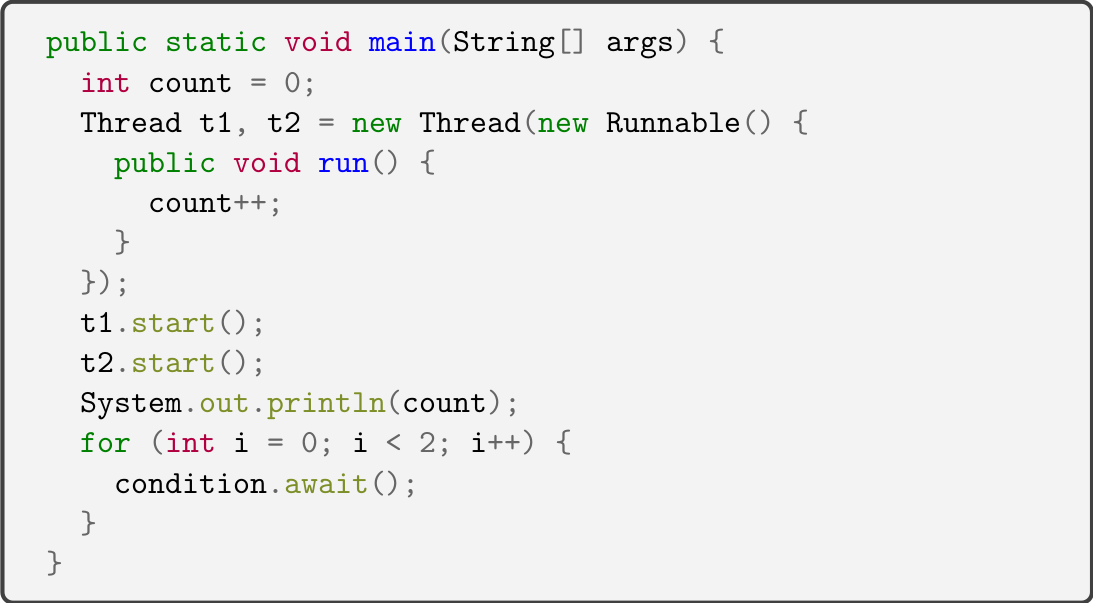
\includegraphics[width=0.9\textwidth]{uno.png}\\

Veamos a la instrucción de la línea 7, $count++$, como: 
\begin{lstlisting}
	int temp = counter;
	counter = temp + 1;
\end{lstlisting}


\begin{itemize}
\item[•] Condición de Carrera:\\
Por lo cual la instrucción genera una condición de carrera ya el resultado del programa será diferente dependiendo del orden de la ejecución por los dos hilos.

\item[• ] Condición por los datos:\\
De igual manera la instrucción de la línea 7 genera una condición por los datos, ya que ambos hilos acceden al valor de la variable $count$ lo leen y existe una escritura cuando se reasigna el valor de la misma.

\item[• ] Otro:

\item[• ] Otro:

\end{itemize}


\item[2. ] Utilizando únicamente semáforos crea una estructura de datos concurrente que
pueda guardar N objetos, y que implemente la siguiente interfaz:\\

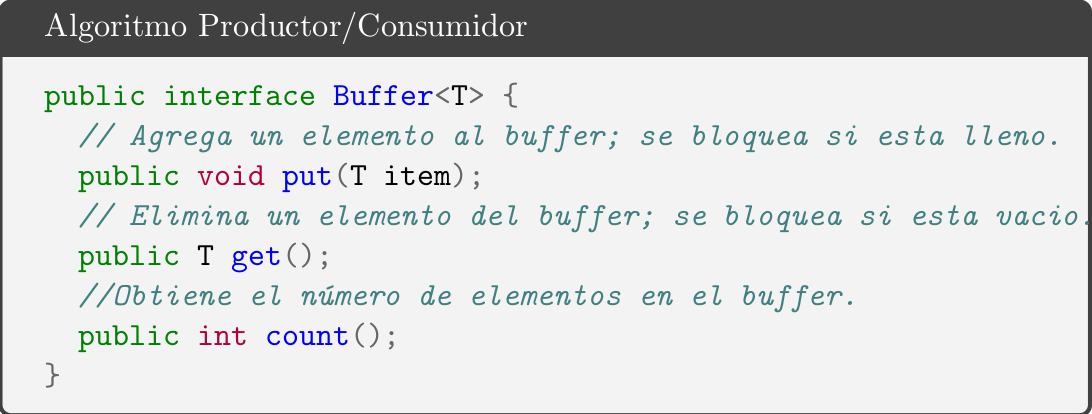
\includegraphics[width=0.9\textwidth]{dos.png}\\
Creamos la estructura de la siguiente manera:
\begin{lstlisting}
public class Estrucutura implements Buffer<T>{

    BoundeQueue<T> e = new BoundeQueue<T>(N);
    Semaphore usarE = new Semaphore(1);
    Semaphore emptyE = new Semaphore(n); // Lugares libres
    Semaphore fullE = new Semaphore(0); // Lugares ocupados

    public void put(T item) {
        emptyE.acquire();   // Vemos si podemos tomar
        usarE.acquire();    // Para poder usar SC
        e.put(item);    
        fullE.release();    // Hay un lugar mas ocupado
        usarE.release();    // Ya no usamos SC
    }

    public T get() {
        T item;
        fullE.acquire();    // Vemos si hay almenos un elemento
        usarE.acquire();    // Para poder usar SC
        item = e.get();  
        emptyE.release();   // Mostramos que quitamos un elemento
        usarE.release       // Ya no usamos SC
        return item;
    }

    public int count(){
        return e.size();
    }
}
\end{lstlisting}



\item[3. ]Utilizando la misma interfaz del ejercicio 1, da una implementación pero ahora
utilizando únicamente candados y condiciones. ¿Tu implementación sufre del
problema del despertar perdido? Argumenta porque no, o muestra un escenario
en donde suceda.

\begin{lstlisting}
public class Estrucutura implements Buffer<T>{
    BoundeQueue<T> e = new BoundeQueue<T>(N);
    ReentrantLock usarE = new ReentrantLock();
    Condition fullE = usarE.newCondition(); 
    Condition emptyE = usarE.newCondition();

    public void put(T item) {
        usarE.lock();
        while (e.isFull()) { // Si E esta llena esperamos
            fullE.await();
        }
        e.put(item); 
        emptyE.signal();	// Al agregar un elemento avisamos que ya no es vacia
        usarE.unlock();
    }

    public T get() {
        T item;
        usarE.lock();
        while(e.isEmpty()){	// Si E esta vacia esperamos
            emptyE.await();
        }
        item = e.get();
        fullE.signal();	// Al quitar un elemento avisamos que ya no esta llena
        usarE.unlock();
        return item;
    }

    public int count(){
        return e.size();
    }
}
\end{lstlisting}

Esta implementación no sufre el problema del despertar perdido, ya que en cada adición de un elemento en la estructura justo la siguiente instrucción es mandar un signal para indicar que ya hay al menos un elemento más ( en caso de que alguien quiera tomar uno). De igual manera si quitamos un elemento la siguiente instrucción es avisar que al menos hay un elemento menos (en caso de que alguien quiera agregar otro). Por lo que hacemos tantos $\textbf{Signal}$ como elementos agregamos o quitamos por lo que avisamos en todo momento a los hilos que esten esperando en una u otra cola de condición.

\item[4. ]Demuestra que en el candado $\textbf{ReadWriteLock}$ visto en clase, cuando un lector
ejecuta $\textbf{signalAll}$ solo puede haber hilos escritores bloqueados.

Tenemos los sigueinte:

\begin{minipage}{0.45\linewidth}
\begin{lstlisting}
// Readers

public void lock(){
	mutex.lock();
	while(writer){
		condition.await();
	}
	readAcquires++;
	mutex.unlock();
}

public void unlock(){
	mutex.lock();
	readers--;
	if(readers == 0){
		condition.signalAll();
	}
	mutex.unlock();
}
\end{lstlisting}
\end{minipage}
\hfill
\begin{minipage}{0.45\linewidth}
\begin{lstlisting}
// Writers

public void lock(){
	mutex.lock();
	while(writer){
		condition.await();
	}	
	writer = true;
	while(readAcquires != readReleases){
		condition.await();
	}
	mutex.unlock();
}

public void unlock(){
	mutex.lock();
	writer = false;
	condition.signalAll();
	mutex.unlock();
}

\end{lstlisting}
\end{minipage}

\item[5. ][2 pts] En clase vimos que la implementación de la estructura SimpleBoard le
da prioridad a los lectores. Posteriormente, discutimos una implementación que
utiliza spin-locks para darle prioridad a los escritores. Modifica la estructura
SimpleBoard para que ahora únicamente use semáforos. Argumenta porque no
puede haber un escritor y lector dentro de la S.C. Hint: Utiliza 4 semáforos
binarios, dos de ellos para proteger las escrituras a las variables y los otros 2
para controlar la entrada de los lectores y escritores.

\item[6. ]Escribe un código genérico utilizando semáforos (de preferencia muy corto)
para un hilo tk de manera que se pueda producir inanición (suponiendo que
todos los hilos ejecutan el mismo código) si los semáforos son débiles, pero no
podría ocurrir si los semáforos son fuertes. Tu código no debe tener deadlocks,
independientemente del tipo de semáforo que se utilice.


\begin{lstlisting}
public class SimpleBoard<T>(){

private int readers = 0;
private semaphore emptySC = new Semaphore(1);
private T message;
private Semaphore permiteLector = new Semaphore(1);


public void write (T msg){
	emptySC.acquire();
	message = msg;
	emptySC.realease();

} 

public void read(){
	permiteLector.acquire();
	if(readers == 0) emptySC.acquire();
	readers ++;
	permiteLector.realease();

}

}

\end{lstlisting}


Para este caso un hilo $t_{k}$ muere de inanicion si un semaforo es debil ya que los semaforos debiles tienen la caracteristica de mandar cualquier hilo osea que no cumplen la caracteriztica de justicia, en los semaforos fuertes van entrando de una manera ordenada en este caso el hilo $t_{k}$ no muere de inanicion ya que en el turno k pasara.



\item[7. ]Considera el siguiete código:\\

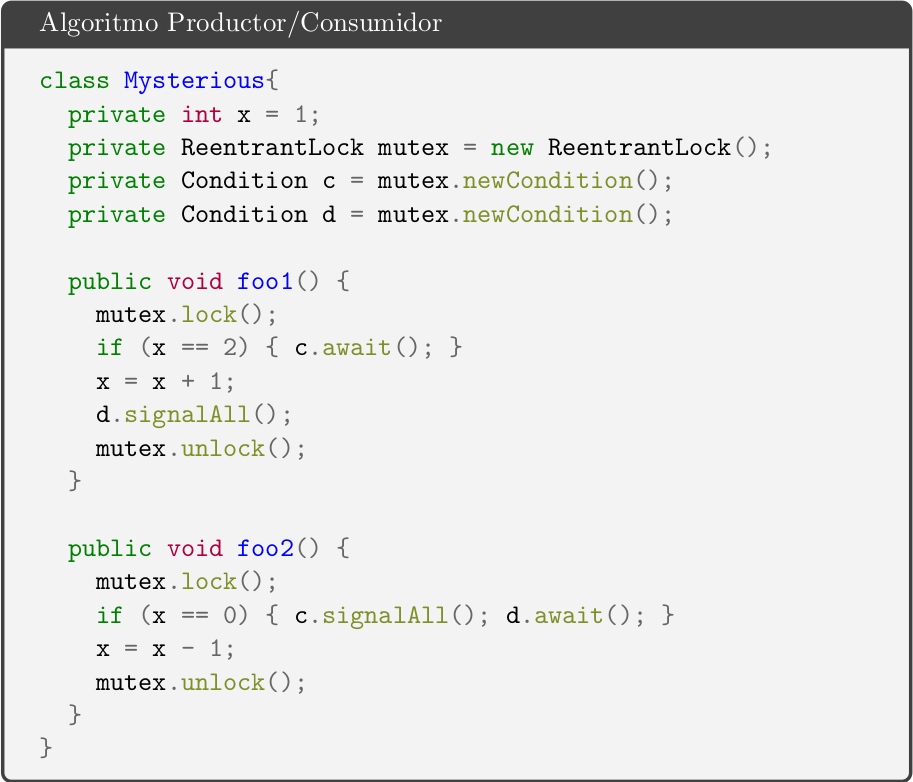
\includegraphics[width=0.9\textwidth]{siete.png}\\
\begin{itemize}
\item[a) ]Demuestra que no tiene deadlocks bajo el supuesto de que los hilos invocan infinitamente los métodos foo1() y foo2().

Supongamos que existe un deadlook entonces los hilos se encolan en c y d para esto la variable x tiene que tener el valor de 2 y de 0 al mismo tiempo notemos que esto no es posible ya que el candado aseguira la exclusion mutua para la variable compartida x.

\item[b) ]Supón ahora que el sistema incluye únicamente los hilos t, u, v. Describe
un escenario en donde el hilo t en algún punto muere de inanición. Ningún
hilo falla, por lo que el calendarizador puede ejecutarlos en cualquier
momento.

En esta ejecucion consiste en atorar a t en la cola c y mantener con los hilos u y v el valor de $x > 0$ para que el hilo t nunca despierte.


\begin{center}



\begin{tabular}{|c|c|c|c|}
\hline 
hilo t & hilo c & hilo v & memoria \\ 
\hline 
 &  &  & x =1 \\ 
\hline 
foo1, x = x+1 &  &  & x = 2 \\ 
\hline 
foo1 , read(x),c.wait() &  &  & x =2 \\ 
\hline 
 & foo2,x = x-1 &  & x = 1 \\ 
\hline 
 &  & foo1,x =x+1 & x = 2 \\ 
\hline 
 & foo2, x = x-1 &  & x = 1 \\ 
\hline 
 &  & foo1,x =x+1 &  x = 2 \\ 
\hline 
 & foo2, x = x-1 &  & x = 1 \\ 
\hline 
\end{tabular} 

\end{center}


\end{itemize}

\newpage

\item[8. ]Otra manera de resolver el problema de la barrera reutilizable para N hilos
es la siguiente: Un hilo especial llamado manager espera por todos los hilos
participantes a que lleguen a la barrera. Cuando todos llegan les devuelve la
señal a todos. Muestra un algoritmo que implemente esta misma idea utilizando
semáforos y demuestra que ningún hilo puede traspasar la barrera dos o más
veces seguidas.
\begin{lstlisting}

public void enter(){
	syncronized(this){
		thread.manager.wakeup();
		if(thread.name == Manager){
			while(haveEnter != N){
				thread.sleep();			
			}
				gate.release();
				notifyAll();			
					
		}	
	}else{
		if(semaphores[thread.ID].getValue()<1){
			semaphores[thread.ID].release();
			haveenter++;		
		}else{
			wait();		
		}
	}
}


\end{lstlisting}

\begin{lstlisting}

public void leave(){
	syncronized(this){
		if(thread.name = manager){
			while(haveEneter != 0){
				thread.sleep();			
			}	
			gate.acquire();
		}else{
			if(semaphores[thread.ID].getValue > 0){
				semaphores[thread.ID].acquire();
				haveEneter--;			
			}
		}
	}
}

\end{lstlisting}

Para esta solucion utilizamos un arreglo de semaforos donde cada hilo tiene un semaforo para entrar a la barrera el hilo manager verifica el numero de hilos que han dado permiso a su propio semaforo una vez que todos los semaforos estan prendidos entra a la seccion critica, el metodo leave verifica que todos los hilos abandonen la barrera y el hilo manager cierra la puerta para volverla reutilizable.


\end{itemize}

\end{document}
